\documentclass[../main.tex]{subfiles}
\begin{document}
	
	\graphicspath{{AppendixC/}}
	\chapter{Supplementary Material to "Discovery of a cryptic allosteric site in Ebola's 'undruggable' VP35 protein"}
	\label{ch:vp35-supp-info}
	
    \textit{This chapter is adapted from the following publication:}

    \textit{Cruz, M.A.$^*$ and Frederick, T.E.$^*$, Singh, S., Vithani, N., Zimmerman, M.I., Porter, J.R., Moeder, K.E., Amarasinghe, G.K., and Bowman, G.R., Discovery of a cryptic allosteric site in Ebola's 'undruggable' VP35 protein using simulations and experiments. Preprint on BioRxiv https://doi.org/10.1101/2020.02.09.940510}\cite{Cruz2020vp35}
	

\section{Supplementary Material}
    \begin{figure}[!htb] %Positioning code for figure
        \centering
        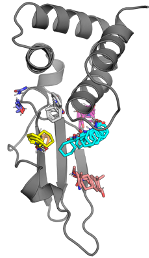
\includegraphics[width=1.5in]{ch5-suppfig1.png}
        \caption[FTMap results for the main cryptic pocket highlighting an example protein structure and hotspots where a variety of small organic probes form energetically favorable interactions.]
            {FTMap results for the main cryptic pocket highlighting an example protein structure (gray) and hotspots where a variety of small organic probes (multicolored sticks) form energetically favorable interactions. The probe molecules are intended to capture different drug-like interactions (such as hydrogen bonding and Van der Waals contacts) and include acetamide, acetonitrile, acetone, acetaldehyde, methylamine, benzaldehyde, benzene, isobutanol, cyclohexane, N,N-dimethylformamide, dimethyl ether, ethanol, ethane, phenol, isopropanol, or urea.}
        \label{fig:ch5-suppfig1}
    \end{figure}

    \begin{figure}[!htb] %Positioning code for figure
        \centering
        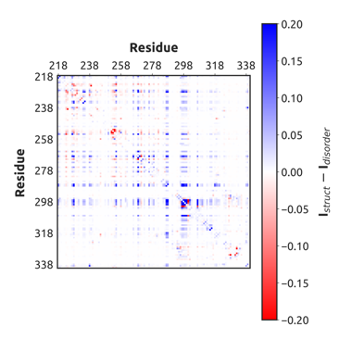
\includegraphics[width=2.5in]{ch5-suppfig2.png}
        \caption[Purely structural correlations dominate the eVP35 allosteric network.]
            {Purely structural correlations ($I_struct$) dominate the allosteric network identified by CARDS as they are typically greater than the disorder-mediated couplings ($I_disorder$, which includes correlations between the structure of one residue and the disorder of a second, as well as correlations between the disorder of two residues).}
        \label{fig:ch5-suppfig2}
    \end{figure}


    \begin{figure}[!htb] %Positioning code for figure
        \centering
        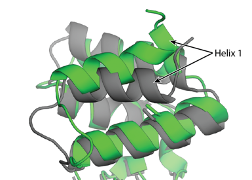
\includegraphics[width=1.5in]{ch5-suppfig3.png}
        \caption[Motion of helix 1 sometimes exposes C247 to solvent.]
            { Motion of helix 1 (green vs gray structures) sometimes exposes C247 (sticks) to solvent. However, the resulting pocket is small and FTMAP does not identify any hotspots in this region that are likely to bind drug-like molecules. Therefore, we focus our attention on the cryptic pocket created by the displacement of helix 7.}
        \label{fig:ch5-suppfig3}
    \end{figure}

    \begin{figure}[!htb] %Positioning code for figure
        \centering
        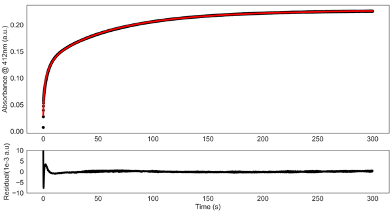
\includegraphics[width=1.5in]{ch5-suppfig4.png}
        \caption[A representative time trace from a thiol labeling experiment ]
            {A representative time trace from a thiol labeling experiment (black) performed at 100 $\mu$M DTNB and a quadruple exponential fit (red). The data are background subtracted (e.g. the average absorbance from three runs with DTNB but no protein were subtracted) to account for spontaneous hydrolysis of DTNB.}
        \label{fig:ch5-suppfig4}
    \end{figure}

    \begin{figure}[!htb] %Positioning code for figure
        \centering
        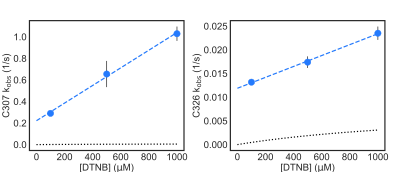
\includegraphics[width=1.5in]{ch5-suppfig5.png}
        \caption[Thiol labeling of a C247S/C275S variant that only has cysteines in the main cryptic pocket.]
            {Thiol labeling of a C247S/C275S variant that only has cysteines in the main cryptic pocket (C307, left and C326, right). Observed labeling rates (blue circles) are shown at a range of DTNB concentrations. Fits to the Linderstrøm-Lang model are shown in dashed colored lines and the expected labeling rate from the unfolded state is shown as black dotted lines. The mean and standard deviation from three replicates are shown but error bars are generally smaller than the symbols.}
        \label{fig:ch5-suppfig5}
    \end{figure}

    \begin{figure}[!htb] %Positioning code for figure
        \centering
        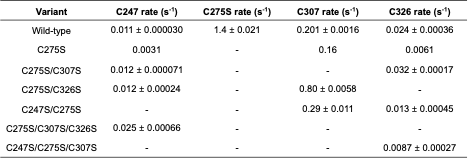
\includegraphics[width=4in]{ch5-suppfig6.png}
        \caption[Observed labeling rates at 100 $\mu$M DTNB for a set of variants.]
            {Observed labeling rates at 100 $\mu$M DTNB for a set of variants with different cysteines mutated to serines to uncover which rate in the wild-type fit corresponds to which cysteine residue. Error is standard deviation from three replicates. Dash represents rates not measured due to the absence of that cysteine residue.}
        \label{fig:ch5-suppfig6}
    \end{figure}

    \begin{table}[]
    \centering
    \caption[Characterization of the folding/unfolding of VP35’s IID]{Characterization of the folding/unfolding of VP35’s IID used to test whether the observed thiol labeling is due to fluctuations within the native state or global unfolding of the protein. K is the equilibrium constant between the folded and unfolded state determined from denaturation data, kunfold is the unfolding rate of the respective variants measured by intrinsic tryptophan fluorescence.}
    \label{tab:ch5-supptab1}
    \begin{tabular}{|l|l|l|}
    Variant     & K                     & K$_{unfold}$(s$^{-1}$) \\
    Wild-type   & 6.57$\times$10$^{-5}$ $\pm$ 4.0$\times$10$^{-5}$ & 0.0175         \\
    C247S/C275S & 4.01$\times$10$^{-4}$ $\pm$ 0.8$\times$10$^{-4}$ & 0.0083        
    \end{tabular}
    \end{table}

    \begin{table}[]
    \centering
    \caption[Intrinsic labeling rates (k$_{int}$) for each cysteine residue.]{Intrinsic labeling rates (k$_{int}$) for each cysteine residue. Intrinsic labeling rates were measured using either urea unfolded variants containing only the specified cysteine, or peptides containing the specified cysteine and its surrounding residues.}
    \label{tab:ch5-supptab2}
    \begin{tabular}{ll}
    \hline
    Residue & kint$\mu$M$^{-1}$s$^{-1}$      \\ \hline
    C247    & 0.0566 $\pm$ 0.0007 \\ \hline
    C275    & 0.00254 $\pm$ 0.001 \\ \hline
    C307    & 0.0290 $\pm$ 0.002  \\ \hline
    C326    & 0.395 $\pm$ 0.02    \\ \hline
    \end{tabular}
    \end{table}

    \begin{figure}[!htb] %Positioning code for figure
        \centering
        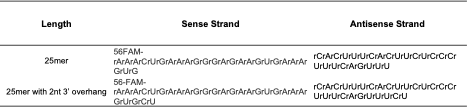
\includegraphics[width=5in]{ch5-suppfig7.png}
        \caption[RNA sequences used in fluorescence polarization binding assays.]
            {RNA sequences used in fluorescence polarization binding assays. The sense and antisense strands were annealed in a 1:1 molar ratio}
        \label{fig:ch5-suppfig7}
    \end{figure}

    \begin{figure}[!htb] %Positioning code for figure
        \centering
        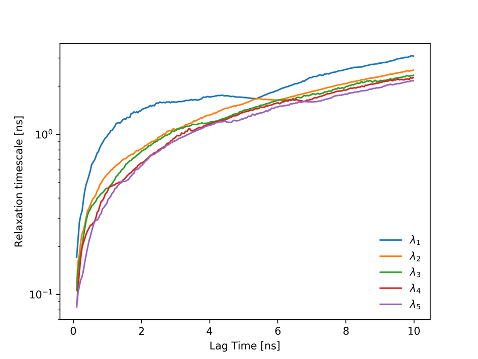
\includegraphics[width=4in]{ch5-suppfig8.png}
        \caption[Implied timescales test for the VP35 IID MSM.]
            {Implied timescales test for the VP35 IID MSM suggests the kinetics are stable from 3-6ns. Analysis in the main text uses a Markov time of 6 ns. Key results were consistent for lag times from 3-6 ns.}
        \label{fig:ch5-suppfig8}
    \end{figure}


	
	
\end{document}